\chapter{Opracowanie koncepcji systemu}
\label{cha:koncepcjaSystemu}
Rozdział ten w dwóch podrozdziałach przedstawia koncepcję implementowanej aplikacji. W podrozdziale pierwszym opisany jest system, w drugim znajduje się specyfikacja wymagań. Dokumentacja projektu zawarta w tym rozdziale oraz w \ref{projektSystemu} została częściowo oprata na szablonie dokumentacji projektu stworzonym przez dr Piotra Szweda \cite{DOC01}.
\section{Opis systemu}
W tym podrozdziale opisany jest cel systemu, jego granice, lista możliwości systemu oraz jego użytkownicy. Ponadto za pomocą diagramów aktywności przedstawione jest działanie aplikacji.
\subsection{Cel projektu}
Celem projektu jest implementacja serwisu internetowego dedykowanego dla studentów w architekturze SOA. Głównym zadaniem serwisu ma być możliwość przechowywania plików oraz udostępnianie ich innym użytkownikom. Ponadto każdy z użytkowników będzie mógł korzystać z dedykowanego dla niego kalendarza, w którym może zapisywać ważne wydarzenia. Oprócz opisanych wcześniej funkcji użytkownik za pomocą strony powiadomień będzie mógł się dowiedzieć o nadchodzących wydarzeniach oraz o udostępnionych dla niego plikach.

\subsection{Użytkownicy}
Grupę użytkowników stanowią wszyscy korzystającyz serwisu, z wyszczególnieniem:
\begin{itemize}
	\item \textbf{Użytkownik} - Docelowym użytkownikiem serwisu jest student potrzebujący dodać lub uzyskać dostęp do pliku poprzez udostępnienie od innych użytkowników serwisu. Nie jest warunkiem koniecznym, aby użytkownik był studentem.
	\item \textbf{Administrator} - Użytkownik posiadający szystkie uprawnienia, takie jak usówanie użytkowników oraz wgląd do wszystkich plików w systemie.
\end{itemize}

\subsection{Granice systemu}
Granicą systemu dla użytkownika jak i dla administratora będzie strona internetowa aplikacji. Zawarty będzie tam dostęp do wszystkich funkconalności systemu. Administrator dodatkowo będzie miał dostęp do specjalnego panelu za pomocą którego będzie mógł zarządzać kontami wszystkich użytkowników.

Wejścia w systemie:
\begin{itemize}
	\item formularz nowego konta – użytkownik wypełnia dane: login, hasło, imie, nazwisko, adres e-mail,
	\item formularz logowania – zalogowanie się do systemu za pomocą loginu i hasła użytkownika,
	\item formularz edycji konta – zmiana danych użytkownika,
	\item formularz nowego pliku – załączonik oraz opcjonalnie tytuł i opis pliku,
	\item formularz edycji pliku - zmiana załącznika, tytułu lub opisu,
	\item formularz udostępnienia pliku - login użytkownika, któremu ma być udostępniony wybrany plik,
	\item formularz nowego wydarzenia - wybrana data, nazwa wydarzenia oraz opcjonalny opis,
	\item formularz edycji wydarzenia - nowe dane do wybranego wydarzenia,
\end{itemize}
Wyjścia w systemie:
\begin{itemize}
	\item Strona powiadomień - na tej stronie znajdować się będą informacje o udostępnionych plikach oraz o przypomnienia o nadchodzących wydarzeniach.
	\item Strona przeglądania własnych plików - użytkownik na tej stronie może przeglądać dodane przez siebie pliki,
	\item Strona przeglądania udostępnionych plików - tutaj użytkownik będzie mógł przeglądać pliki mu udostępnione,
	\item Strona kalendarza - Strona odpowiedzialna za wyświetlanie kalendarza.
\end{itemize}
\subsection{Lista możliwości}
\label{listaFun}
\textbf{Lista wymagań funkcjonalnych:}
\begin{itemize}
	\item Logowanie,
	\item Wylogowanie,
	\item Rejestracja,
	\item Zarządzanie kontem,
	\item Zarządzanie materiałami,
	\item Pobieranie pliku,
	\item Udostępnianie pliku,
	\item Zarządzanie kalendarzem,
	\item Otrzymywanie powiadomień,
\end{itemize}

\textbf{Dodatkowe funkcje administratora:}
\begin{itemize}
	\item Zarządzanie kontami użytkowników.
\end{itemize}


\textbf{Na kolejnych stronach zostały przedstawione diagramy czynności typowych akcji.}
	\begin{figure}[H]
	\centering
	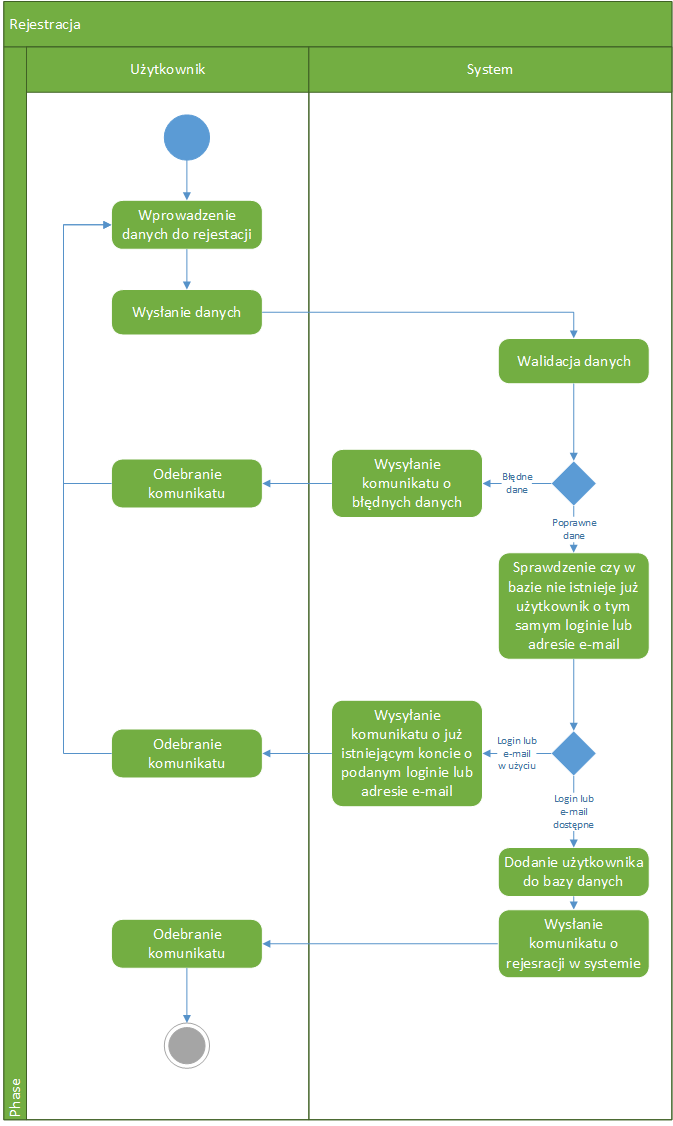
\includegraphics[scale=0.5]{Rejestracja}
	\caption{\label{fig:activity_01}Rejestracja}
	\end{figure}
	\begin{figure}[H]
	\centering
	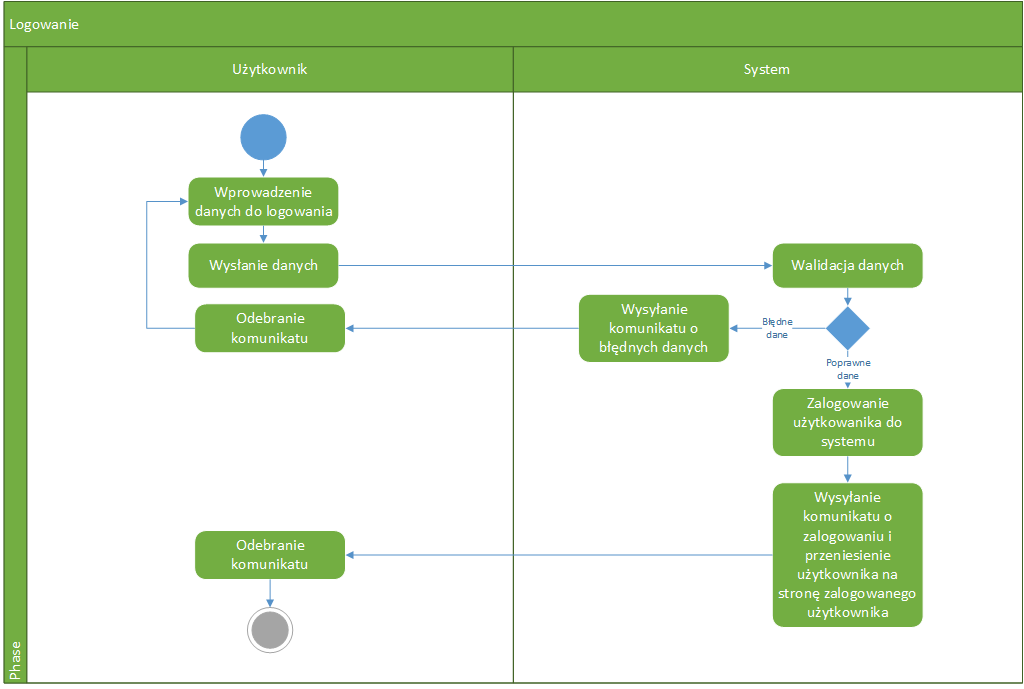
\includegraphics[scale=0.5]{Logowanie}
	\caption{\label{fig:activity_02}Logowanie}
	\end{figure}
	\begin{figure}[H]
	\centering
	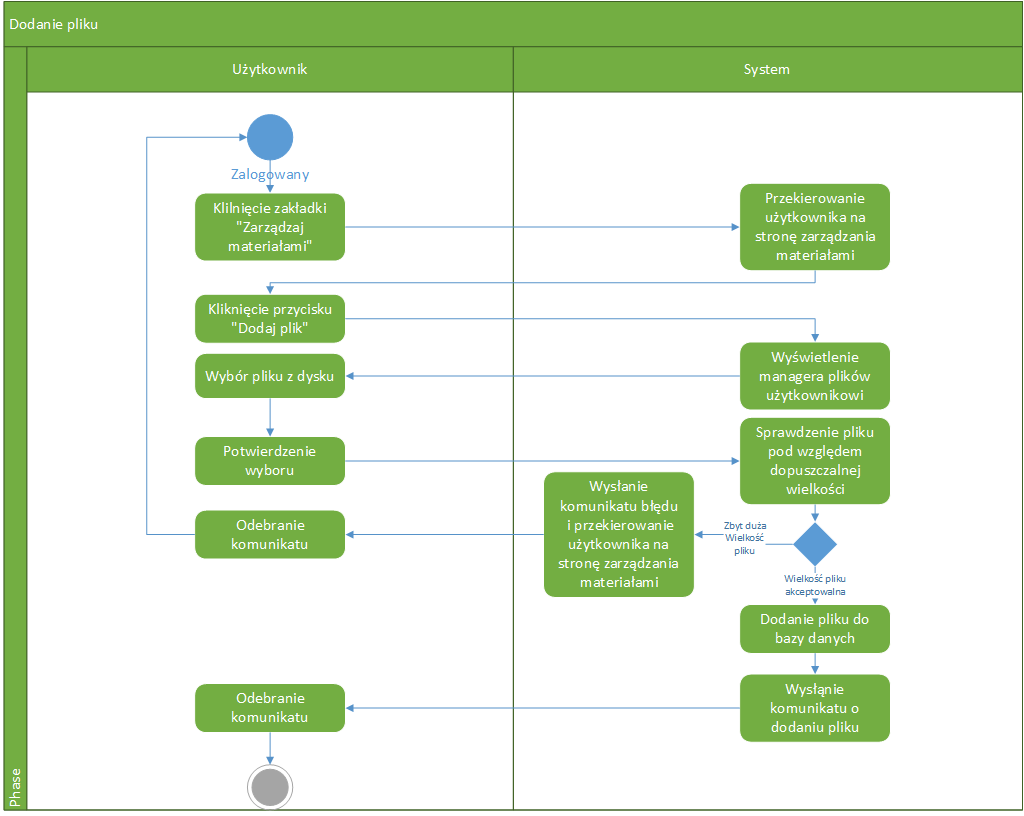
\includegraphics[scale=0.5]{DodaniePliku}
	\caption{\label{fig:activity_03}Dodanie Pliku}
	\end{figure}
	\begin{figure}[H]
	\centering
	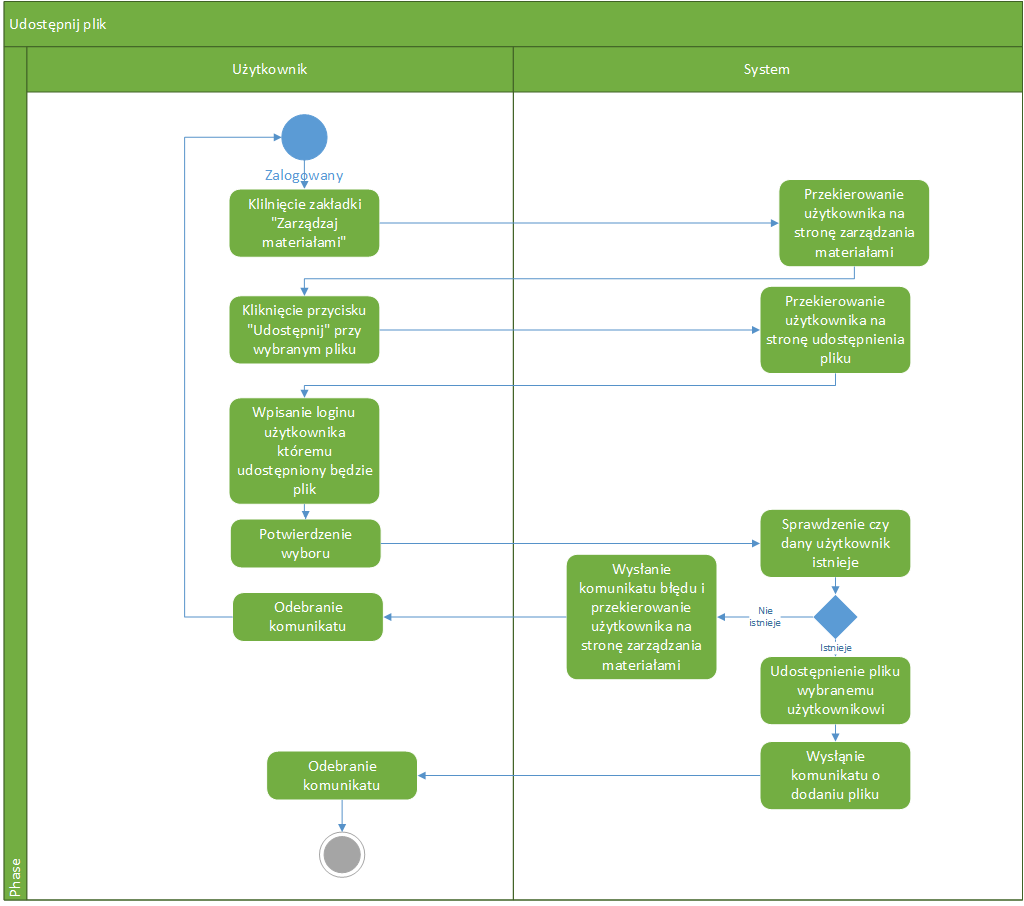
\includegraphics[scale=0.5]{Udostepnienie}
	\caption{\label{fig:activity_04}Udostępnienie Pliku}
	\end{figure}
\section{Specyfikacja i analiza wymagań}
Dzięki analizie wymagań funkcjonalnych możemy zidentyfikować oczekiwane zachowania budowanego systemu. Wymaganie funkcjonalne jest to „stwierdzenie, jakie usługi ma oferować system, jak ma reagować na określone dane wejściowe oraz jak ma się zachowywać w określonych sytuacjach. W niektórych wypadkach wymagania funkcjonalne określają, czego system nie powinien robić” \cite{DOC02}. W tym podrozdziale opisane zostaną lista wymagań wunkonalnych oraz niefunkcjonalnych oraz przedstawiony zostanie diagram przypadków użycia z dołączonymi scenariuszami.
\subsection{Wymagania oprogramowania}
Wymagania funkcjonalne zostały wypisane w podpunkcie \ref{listaFun}.
Wymagania niefunkcjonalne:
\begin{enumerate}
	\item Wymaganie organizacyjne:
		\begin{itemize}
			\item Implementacji : językiem programowania jest Java,
			\item Użyteczności : Interfejs graficzny użytkownika jest przejrzysty i łatwy do przyswojenia,
		\end{itemize}
	\item Wymagania zewnętrzne:		
		\begin{itemize}
			\item Poufności - Projekt przestrzega wymagań prawnych ustanowionych w Ustawie o Ochronie Danych Osobowych.
			\item Bezpieczeństwa : System nie pozwala użytkownikom na nieautoryzowany dostęp do bazy danych
		\end{itemize}
\end{enumerate}
\subsection{Ryzyka operacyjne}
Ryzykiem w implementowanym systemie może być niedostateczne zabezpieczenie bazy danych lub pojawienie się nieobsłużonych błędów.
//TODO: Poszukać i dodać tu jeszcze cos
\subsection{Przypadki użycia}
Dzięki przypadkom użycia możemy okeślić jak użytkownik będzie korzystał z systemu. Dzięki diagramowi możemy zobaczyć jakie czynności może wykonywać dany użytkownik \cite{DOC03}. Opisy czynności zawartych na diagramie znajdują się w scenariuszach przypadków użycia.

Poniższe diagramy prezentują możliwe interakcje użytkowników z systemem.
\begin{figure}[H]
	\centering
	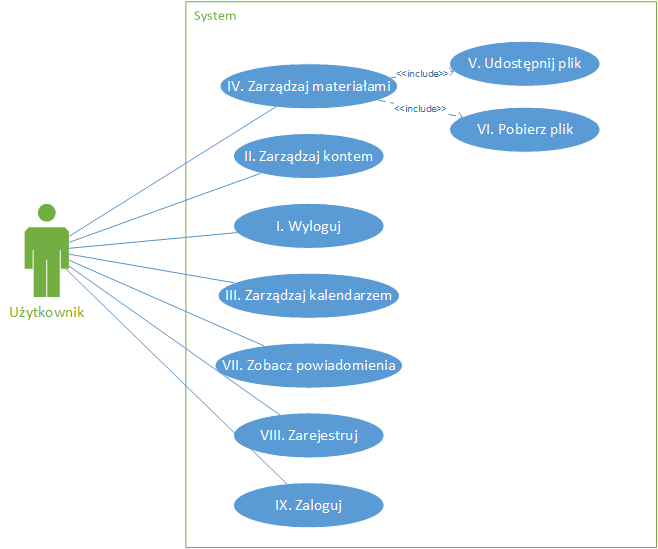
\includegraphics[scale=0.7]{UseCaseUser}
	\caption{\label{fig:caption_01}Diagram przypadków użycia dla użytkownika}
\end{figure}
W poniższym diagramie pominięto przypadki użycia, które posiada zwykły użytkownik, lecz nie należy zapominać, że administrator również je posiada.
\begin{figure}[H]
	\centering
	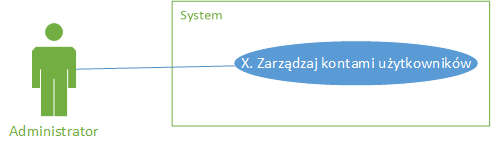
\includegraphics[scale=0.7]{UseCaseAdmin.png}
	\caption{\label{fig:caption_02}Diagram przypadków użycia dla administratora}
\end{figure}

Scenariusze przypadków użycia:
\begin{enumerate}[label=(\Roman*)]
	\item Wyloguj
	\begin{table}[H]
\centering
\caption{Wyloguj}
\label{wyloguj}
\begin{tabular}{|p{7cm}|p{7cm}|}
  \hline 
  \textbf{Aktorzy:} & Użytkownik, Administrator\\
  \hline
  \textbf{Zakres:} & System \\
	\hline
  \textbf{Poziom:} & Sytemowowy \\
	\hline
  \textbf{Udziałowcy i ich cele: } & Użytkownik chce się wylogować. \\
	\hline
  \textbf{Zdarzenie wyzwalające } & Użytkownik wciska przycisk “Wyloguj”. \\
	\hline
  \textbf{Warunki wstępne: } & Użytkownik jest zalogowany.
 \\
	\hline
  \textbf{Warunki końcowe dla sukcesu:} & Użytkownik jest wylogowany.
 \\
	\hline
  \textbf{Warunki końcowe dla niepowodzenia:} & Użytkownik jest zalogowany. \\
  \hline
\end{tabular} 
\end{table}

\textbf{Scenariusz główny:} \\
1. Użytkownik wciska przycisk wyloguj widoczny w prawym górnym rogu strony. \\
2. Pojawia się okno z napisem: “Czy na pewno chcesz się wylogować?” \\
3. Użytkownik wciska przycisk “tak”. \\
4. Użytkownik jest wylogowany i przekierowany na stronę główną systemu. \\
\textbf{Scenariusz alternatywany: \\
} 
3.a. Użytkownik wciska “nie”. \\
3.a.1. Okno z napisem znika, użytkownik dalej jest zalogowany. \\
\item Zarządzaj kontem
\begin{table}[H]
\centering
\caption{Zarządzaj kontem}
\label{zarzadzajkontem}
\begin{tabular}{|p{7cm}|p{7cm}|}
  \hline 
  \textbf{Aktorzy:} & Użytkownik, Administrator\\
  \hline
  \textbf{Zakres:} & System \\
	\hline
  \textbf{Poziom:} & Sytemowowy \\
	\hline
  \textbf{Udziałowcy i ich cele: } & Użytkownik chce zmienić login lub hasło. \\
	\hline
  \textbf{Zdarzenie wyzwalające } & Użytkownik wciska przycisk “Zarządzaj kontem”. \\
	\hline
  \textbf{Warunki wstępne: } & Użytkownik jest zalogowany.\\
	\hline
  \textbf{Warunki końcowe dla sukcesu:} & Login lub hasło użytkownika są zmienione.\\
	\hline
  \textbf{Warunki końcowe dla niepowodzenia:} & Login lub hasło użytkownika nie są zmienione. \\
  \hline
\end{tabular} 
\end{table}

\textbf{Scenariusz główny:}\\
	1. Użytkownik wciska przycisk: “Zarządzaj kontem”.\\
	2. System przenosi użytkownika do strony zarządzania kontem, na której ma do wyboru
	dwie opcje: “Zmień login” i “Zmień hasło”\\
	3. Użytkownik wybiera opcje “Zmień login”.\\
	4. System przenosi użytkownika do strony zmiany loginu, na której znajduje się
	formularz z polem tekstowym na nowy login.\\
	5. Użytkownik wpisuje nowy login i wciska “Zatwierdź”.\\
	6. System sprawdza czy nowy login nie występuje w bazie danych.\\
	7. System wyświetla okno o pomyślnej zmianie loginu i przekierowuje użytkownika do
strony zarządzania kontem.\\
\textbf{Scenariusz alternatywny:}\\
3.a. Użytkownik wybiera opcje “Zmień hasło”.\\
3.a.1. System przenosi użytkownika do strony zmiany hasła, na której znajduje się formularz
z polem tekstowym na nowe hasło.\\
3.a.2. Użytkownik wpisuje nowe hasło w pola “hasło” oraz “potwierdź hasło” i wciska
“Zatwierdź”.\\
3.a.3. System sprawdza czy wartości z pola hasło i potwierdź hasło są takie same.\\
3.a.4. System sprawdza czy hasło ma odpowiednią długość i zawiera duże znaki.\\
3.a.5. System wyświetla komunikat o poprawnej zmianie hasła i przenosi użytkownika do
strony zarządzania kontem.\\
\textbf{Scenariusz alternatywny:}\\
3.a.3.a Wartość z pola hasło i potwirdź hasło nie są takie same.\\
3.a.3.a.1 System wyświetla odpowiedni komunikat błędu
\textbf{Scenariusz alternatywny:}\\
7.b. System wyświetla komunikat błędu: “Podany login już istnieje w systemie”.\\
7.b.1. Powrót do pkt.4 scenariusza głównego.\\

	\item Zarządzaj kalendarzem:
	\begin{table}[H]
\centering
\caption{Zarządzaj kalendarzem}
\label{zarzadzajkalendarzem}
\begin{tabular}{|p{7cm}|p{7cm}|}
  \hline 
  \textbf{Aktorzy:} & Użytkownik, Administrator\\
  \hline
  \textbf{Zakres:} & System \\
	\hline
  \textbf{Poziom:} & Sytemowowy \\
	\hline
  \textbf{Udziałowcy i ich cele: } & Użytkownik chce dodać lub usunąć wydarzenie w kalendarzu. \\
	\hline
  \textbf{Zdarzenie wyzwalające } & Użytkownik wciska przycisk “Zarządzaj kalendarzem”. \\
	\hline
  \textbf{Warunki wstępne: } & Użytkownik jest zalogowany.
 \\
	\hline
  \textbf{Warunki końcowe dla sukcesu:} & Użytkownik dodał, edytował lub usunął wydarzenie.
 \\
	\hline
  \textbf{Warunki końcowe dla niepowodzenia:} & Użytkownik nie dodał, nie edytował lub nie usunął wydarzenia \\
  \hline
\end{tabular} 
\end{table}

\textbf{Scenariusz główny:}\\
1. Użytkownik wciska przycisk “Zarządzaj kalendarzem”.\\
2. System przekierowuje użytkownika na stronę zarządzania kalendarzem.\\
3. Użytkownik wybiera datę w kalendarzu.\\
4. System podświetla wybrany przez użytkownika dzień i wyświetla przycisk “dodaj
wydarzenie”, “usuń wydarzenie” oraz “edytuj wydarzenie”, jeżeli w danym dniu jest
jakieś zapisane.\\
5. Użytkownik wciska przycisk “dodaj wydarzenie”.\\
6. System przenosi użytkownika na stronę dodawania wydarzenia, na której znajduje się
data, pole tekstowe na nazwe wydarzenia oraz na godzinę wydarzenia i czas trwania.\\
7. Użytkownik wypełnia formularz i wciska przycisk “zatwierdź”.\\
8. System sprawdza poprawność wpisanych danych.\\
9. Wydarzenie jest dodane do kalendarza\\
\textbf{Scenariusz alternatywny:}\\
1.b. System wyświetla komunikat błędu: “Błąd serwera”\\
1.b.1. Powrót do pkt.1 scenariusza głównego.\\
\textbf{Scenariusz alternatywny:}\\
8.a. System wyświetla komunikat błędu: “Pole “czas trwania” musi być wypełnione liczbą.”\\
8.a.1. Powrót do pkt. 4 scenariusza głównego.\\
\textbf{Scenariusz alternatywny:}\\
4.a Użytkownik wciska przycisk “usuń wydarzenie”.\\
4.a.1 System przenosi użytkownika na stronę usuwania wydarzenia, na której znajduje się
lista wydarzeń zaplanowanych na wybrany dzień oraz przyciski “usuń” obok każdego z nich.\\
4.a.2 Użytkownik wciska przycisk “usuń” obok jednego z wydarzeń.\\
4.a.3 System wyświetla okno z pytaniem czy na pewno usunąć wydarzenie.\\
4.a.4 Użytkownik wciska przycisk “tak”.\\
4.a.5 System usuwa wydarzenie i wyświetla komunikat o pomyślnym usunięciu wydarzenia.\\
4.a.6 System przekierowuje użytkownika na stronę zarządzania kalendarzem.\\
\textbf{Scenariusz alternatywny:}\\
4.a.3.a Użytkownik wciska przycisk “nie”.\\
4.a.3.a.1 Powrót do pkt. 4 scenariusza głównego.\\
\textbf{Scenariusz alternatywny:}
4.b Użytkownik wciska przycisk “edytuj wydarzenie”.\\
4.b.1 System przenosi użytkownika na stronę edycji wydarzenia, na której znajduje się lista
wydarzeń zaplanowanych na wybrany dzień oraz przyciski “edytuj” obok każdego z nich.\\
4.a.2 Użytkownik wciska przycisk “edytuj” obok jednego z wydarzeń.\\
4.a.3 System wyświetla okno z pytaniem czy na pewno usunąć wydarzenie.\\
4.a.4 Użytkownik wciska przycisk “tak”.\\
4.a.5 System usuwa wydarzenie i wyświetla komunikat o pomyślnym usunięciu wydarzenia.\\
4.a.6 System przekierowuje użytkownika na stronę zarządzania kalendarzem.\\

\item Zarządzaj materiałami:
	\begin{table}[H]
\centering
\caption{Zarządzaj materiałami}
\label{zarządzajmaterialami:}
\begin{tabular}{|p{7cm}|p{7cm}|}
  \hline 
  \textbf{Aktorzy:} & Użytkownik, Administrator\\
  \hline
  \textbf{Zakres:} & System \\
	\hline
  \textbf{Poziom:} & Sytemowowy \\
	\hline
  \textbf{Udziałowcy i ich cele: } & Użytkownik chce dodać, usunąć, pobrać, lub udostępnić plik. \\
	\hline
  \textbf{Zdarzenie wyzwalające } & Użytkownik wciska przycisk “Zarządzaj materiałami”. \\
	\hline
  \textbf{Warunki wstępne: } & Użytkownik jest zalogowany.
 \\
	\hline
  \textbf{Warunki końcowe dla sukcesu:} &Użytkownik dodał, usunął, pobrał, lub udostępnił plik.
 \\
	\hline
  \textbf{Warunki końcowe dla niepowodzenia:} & Użytkownik pozostał na dotychczasowej stronie. \\
  \hline
\end{tabular} 
\end{table}

\textbf{Scenariusz główny:}\\
1. Użytkownik wciska przycisk “zarządzaj materiałami”.\\
2. System przekierowuje użytkownika na stronę zarządzania materiałami.\\
3. Użytkownik wciska przycisk “dodaj plik”.\\
4. System wyświetla nowe okno z eksplorerem plików w celu wybrania pliku z
lokalnego dysku użytkownika.\\
5. Użytkownik wybiera plik i zatwierdza wybór.\\
6. System sprawdza czy plik nie jest zbyt duży.\\
7. System dodaje plik do bazy i wyświetla informacje o pomyślnym dodaniu pliku do
bazy.\\
8. Nowy plik pojawia się w oknie zarządzania materiałami.\\
\textbf{Scenariusz alternatywny:}\\
6.a. System wyświetla komunikat błędu: “Plik zbyt duży.”\\
\textbf{Scenariusz alternatywny:}\\
1.a. System wyświetla komunikat “Błąd serwera”.\\
1.a.1. Użytkownik pozostaje na dotychczasowej stronie.\\
\textbf{Scenariusz alternatywny:}\\
2.a Użytkownik wybiera plik z listy plików użytkownika.\\
2.a.1 System otwiera stronę zarządzania plikiem z informacją o wybranym pliku, oraz trzema
przyciskami: “Usuń”, “Pobierz” oraz “Udostępnij”.\\
2.a.2 Użytkownik wybiera opcję “Usuń”.\\
2.a.3. System wyświetla okno “Czy na pewno chcesz usunąć plik?”.\\
2.a.4 Użytkownik wciska przycisk “tak”.\\
2.a.5 Plik zostaje usunięty z systemu.\\
2.a.6 System przekierowuje użytkownika do strony zarządzania materiałami.\\
\textbf{Scenariusz alternatywny:}\\
2.a.3.a Użytkownik wybiera opcje “nie”.\\
2.a.3.a.1 Powrót do pkt 2 scenariusza głównego.\\

\item Udostępnij plik:
	\begin{table}[H]
\centering
\caption{Udostępnij plik}
\label{Udostepnijplik}
\begin{tabular}{|p{7cm}|p{7cm}|}
  \hline 
  \textbf{Aktorzy:} & Użytkownik, Administrator\\
  \hline
  \textbf{Zakres:} & System \\
	\hline
  \textbf{Poziom:} & Sytemowowy \\
	\hline
  \textbf{Udziałowcy i ich cele: } & Użytkownik chce udostępnić plik. \\
	\hline
  \textbf{Zdarzenie wyzwalające } & Użytkownik wciska przycisk “udostępnij plik”. \\
	\hline
  \textbf{Warunki wstępne: } & Użytkownik jest zalogowany. Użytkownik jest na stronie zarządzania materiałami.
 \\
	\hline
  \textbf{Warunki końcowe dla sukcesu:} & Plik został udostępniony.
 \\
	\hline
  \textbf{Warunki końcowe dla niepowodzenia:} & Plik nie został udostępniony. \\
  \hline
\end{tabular} 
\end{table}

\textbf{Scenariusz główny:}\\
1. Użytkownik wybiera plik z listy.\\
2. System otwiera stronę zarządzania plikiem z informacją o wybranym pliku, oraz trzema przyciskami: “Usuń”, “Pobierz” oraz “Udostępnij”.\\
3. Użytkownik wybiera opcję “Udostępnij”.\\
4. System otwiera stronę udostępniania pliku, na której znajduje się formularz, z polem na nazwę użytkownika oraz przycisk “zatwierdź”.\\
5. Użytkownik wpisuję nazwę użytkownika i wciska przycisk “zatwierdź”.\\
6. System po znalezieniu użytkownika w bazie udostępnia plik wybranemu użytkownikowi.\\
7. System wyświetla wiadomość o pomyślnym udostępnieniu pliku.\\
\textbf{Scenariusz alternatywny:}\\
5.a. System nie znajduje użytkownika w bazie.\\
5.a.1. System wyświetla komunikat o niepowodzeniu.\\

\item Pobierz plik:
	\begin{table}[H]
\centering
\caption{Pobierz plik}
\label{Pobierzplik}
\begin{tabular}{|p{7cm}|p{7cm}|}
  \hline 
  \textbf{Aktorzy:} & Użytkownik, Administrator\\
  \hline
  \textbf{Zakres:} & System \\
	\hline
  \textbf{Poziom:} & Sytemowowy \\
	\hline
  \textbf{Udziałowcy i ich cele: } & Użytkownik chce pobrać plik. \\
	\hline
  \textbf{Zdarzenie wyzwalające } & Użytkownik wciska przycisk “pobierz plik”. \\
	\hline
  \textbf{Warunki wstępne: } & Użytkownik jest zalogowany. Użytkownik jest na stronie zarządzania materiałami.
 \\
	\hline
  \textbf{Warunki końcowe dla sukcesu:} & Plik został pobrany.\\
	\hline
  \textbf{Warunki końcowe dla niepowodzenia:} & Plik nie został pobrany. \\
  \hline
\end{tabular} 
\end{table}

\textbf{Scenariusz główny:}\\
1. Użytkownik wybiera plik z listy.\\
2. System otwiera stronę zarządzania plikiem z informacją o wybranym pliku, oraz trzema przyciskami: “Usuń”, “Pobierz” oraz “Udostępnij”.\\
3. Użytkownik wybiera opcję “Pobierz”.\\
4. System rozpoczyna pobieranie pliku do domyślnego folderu na lokalnej maszynie użytkownika.\\
5. System zakończył pobieranie pliku i wyświetla komunikat o powodzeniu.\\
\textbf{Scenariusz alternatywny:}\\
4.a. System nie może pobrać pliku, ponieważ nastąpiło rozłączenie z serwerem.\\
4.a.1. System wyświetla komunikat o niepowodzeniu.\\

\item Zobacz powiadomienia:
	\begin{table}[H]
\centering
\caption{Zobacz powiadomienia}
\label{Zobaczpowiadomienia}
\begin{tabular}{|p{7cm}|p{7cm}|}
  \hline 
  \textbf{Aktorzy:} & Użytkownik, Administrator\\
  \hline
  \textbf{Zakres:} & System \\
	\hline
  \textbf{Poziom:} & Sytemowowy \\
	\hline
  \textbf{Udziałowcy i ich cele: } & Użytkownik chce zobaczyć powiadomienia. \\
	\hline
  \textbf{Zdarzenie wyzwalające } & Użytkownik wciska przycisk “Zobaczpowiadomienia”. \\
	\hline
  \textbf{Warunki wstępne: } & Użytkownik jest zalogowany. 
 \\
	\hline
  \textbf{Warunki końcowe dla sukcesu:} & Użytkownik znajduje się na stronie powiadomień.\\
	\hline
  \textbf{Warunki końcowe dla niepowodzenia:} & Użytkownik pozostał na dotychczasowej stronie. \\
  \hline
\end{tabular} 
\end{table}
\textbf{Scenariusz główny:}\\
1. Użytkownik wciska przycisk “Zobacz powiadomienia”.\\
2. System otwiera stronę powiadomień.\\
\textbf{Scenariusz alternatywny:}\\
1.a. System wyświetla błąd.\\
1.a.1. Użytkownik pozostaje na dotychczasowej stronie.\\

\item Zarejestruj:
	\begin{table}[H]
\centering
\caption{Zarejestruj}
\label{Zarejestruj}
\begin{tabular}{|p{7cm}|p{7cm}|}
  \hline 
  \textbf{Aktorzy:} & Użytkownik, Administrator\\
  \hline
  \textbf{Zakres:} & System \\
	\hline
  \textbf{Poziom:} & Sytemowowy \\
	\hline
  \textbf{Udziałowcy i ich cele: } & Niezarejestrowany Użytkownik chce się zarejestrować. \\
	\hline
  \textbf{Zdarzenie wyzwalające } & Niezarejestrowany Użytkownik wciska przycisk "Zarejestruj".\\
	\hline
  \textbf{Warunki wstępne: } & Brak. \\
	\hline
  \textbf{Warunki końcowe dla sukcesu:} & Niezarejestrowany Użytkownik znajduje się na stronie głównej.\\
	\hline
  \textbf{Warunki końcowe dla niepowodzenia:} & Konto nie zostaje stworzone , a użytkownik zostaje poinformowany o niepowodzeniu oraz podane zostają przyczyny błędu np. adres emailjest już wykorzystany lub login jest już zajęty. \\
  \hline
\end{tabular} 
\end{table}

\textbf{Scenariusz główny:}\\
1. System wyświetla formularz rejestracyjny.\\\\
2. Użytkownik wypełnia formularz.\\
3. Użytkownik wciska zatwierdź.\\
4. System sprawdza poprawność danych i unikalność loginu.\\
5. Konto użytkownika zostaje utworzone\\
\textbf{Scenariusz alternatywny:}
4.a System znajduje konto o podanym loginie.\\
4.a.1 System wyświetla ponownie formularz z informacją, że konto o podanym loginie już
istnieje.\\
4.a.2 Powrót do punktu 2 scenariusza głównego.\\
\textbf{Scenariusz alternatywny:}\\
4.b System wykrył polskie znaki w haśle.\\
4.b.1 System wyświetla ponownie formularz z informacją, że nie może być polskich znaków
w haśle\\
4.b.2 Powrót do punktu 2 scenariusza głównego.\\
\textbf{Scenariusz alternatywny:}
2.a Użytkownik odświeża stronę.\\
2.a.1 Użytkownik przekierowany jest na stronę główną serwisu.\\

\item Zaloguj:
	\begin{table}[H]
\centering
\caption{Zaloguj}
\label{Zaloguj}
\begin{tabular}{|p{7cm}|p{7cm}|}
  \hline 
  \textbf{Aktorzy:} & Użytkownik, Administrator\\
  \hline
  \textbf{Zakres:} & System \\
	\hline
  \textbf{Poziom:} & Sytemowowy \\
	\hline
  \textbf{Udziałowcy i ich cele: } & Użytkownik chce się zalogować.
 \\
	\hline
  \textbf{Zdarzenie wyzwalające } & Użytkownik wciska przycisk zaloguj.\\
	\hline
  \textbf{Warunki wstępne: } & Użytkownik musi posiadać konto w systemie. \\
	\hline
  \textbf{Warunki końcowe dla sukcesu:} & Użytkownik znajduje się na stronie głównej.\\
	\hline
  \textbf{Warunki końcowe dla niepowodzenia:} & Użytkownik jest niezalogowany. \\
  \hline
\end{tabular} 
\end{table}

\textbf{Scenariusz główny:}\\
1. System wyświetla formularz logowania.\\
2. Użytkownik wypełnia formularz.\\
3. Użytkownik wciska zatwierdź.\\
4. System sprawdza poprawność danych.\\
5. Użytkownik zostaje zalogowany.\\
\textbf{Scenariusz alternatywny:}\\
4.a System odrzuca wprowadzone dane, ponieważ login lub hasło są nieprawidłowe.\\
4.a.1 System wyświetla ponownie formularz z informacją o błędnym loginie lub haśle.\\
4.a.2 Powrót do punktu 2 scenariusza głównego.\\

\item Zarządzaj kontami użytkowników:
	\begin{table}[H]
\centering
\caption{Zarządzaj kontami użytkowników}
\label{zku}
\begin{tabular}{|p{7cm}|p{7cm}|}
  \hline 
  \textbf{Aktorzy:} & Administrator\\
  \hline
  \textbf{Zakres:} & System \\
	\hline
  \textbf{Poziom:} & Sytemowowy \\
	\hline
  \textbf{Udziałowcy i ich cele: } & Administrator chce usunąć, lub edytować konto użytkownika.
 \\
	\hline
  \textbf{Zdarzenie wyzwalające } & Administrator wciska przycisk “zarządzaj kontami”.
\\
	\hline
  \textbf{Warunki wstępne: } & Administrator jest zalogowany. \\
	\hline
  \textbf{Warunki końcowe dla sukcesu:} & Konto użytkownika zostało usunięte lub edytowane.\\
	\hline
  \textbf{Warunki końcowe dla niepowodzenia:} &  Konto użytkownika nie zostało usunięte lub edytowane. \\
  \hline
\end{tabular} 
\end{table}

\textbf{Scenariusz główny:}\\
1. Administrator wciska przycisk “zarządzaj kontami”.\\
2. System przekierowuje na stronę zarządzania kontami użytkowników, gdzie
wylistowane są loginy wszystkich użytkowników, a obok nazwy są dwa przyciski:
“usuń” oraz “edytuj” oraz bad listą pole na wpisanie loginu i przycisk do
zatwierdzania.\\
3. Administrator klika “usuń” przy wybranym loginie.
4. System wyświetla komunikat o treści “Czy na pewno chcesz usunąć użytkownika z
bazy danych?” oraz dwie opcje odpowiedzi: “tak” i “nie”.\\
5. Administrator wciska “tak”\\
6. System usuwa użytkownika z bazy danych.\\
7. System wyświetla komunikat o udanej operacji.\\
\textbf{Scenariusz alternatywny:}\\
2.a Administrator wciska “edytuj”.\\
2.a.1 System przekierowuje administratora na stronę edycji użytkownika z formularzem do
edycji.\\
2.a.2 Administrator wprowadza nowe dane i potwierdza zmianę przyciskiem “zatwierdź”.\\
2.a.3 System zmienia dane użytkownika w bazie.\\
2.a.4 System wyświetla komunikat o udanej operacji.\\
2.a.5 Powrót do pkt 2 scenariusza głównego.\\
\textbf{Scenariusz alternatywny:}\\
2.b Administrator wpisuje login w odpowiednie pole i wciska przycisk szukaj\\
2.b.1 System wyświetla tylko użytkownika o podanym loginie.\\
\end{enumerate}
